\chapter{Architecture}
\label{chapter:architecture}

Alcaudon's architecture will be described in this chapter following a top-down
approach. First, a general description of the different components of the system
will be done and later a more detailed description of each on them.

\subsection{General description}

Alcaudon's platform is composed by 3 main units.

\begin{itemize}
\item \textbf{Coordinator node}: This is the main component of the system. It
  coordinates the life cycle of the different components of the cluster such as
  the computing nodes. It is also responsible of performing the scheduling of
  the user defined dataflows given the resources provided by the computing
  nodes. Finally, it is the interface between the cluster and the users, where
  they deploy their dataflow topologies.

\item \textbf{Computing nodes}: These nodes are in charge of executing the
  actual computations provided by Alcaudon's users. These nodes take care of
  storing intermediate results published to streams. They register dynamically
  to the cluster contacting the coordinator node. A deployment can be formed by
  1 computing node up to thousands, this really depends on the needs. Each of
  these nodes provide certain resources to the system, known as
  \textit{computation slots}. The number of slots is configurable, but they
  correlate with the number of available CPU's in the underlying hardware.

\item \textbf{Alcaudon library}: This is the main interface between users
  and the system. In order to use Alcaudon it is necessary to have access to a
  cluster with a coordinator and computing nodes. This interface is provided as
  a library containing the tools to build dataflows, the interfaces to implement
  user defined stream computations and the tools to connect with a particular
  cluster. Since the computations are potentially infinite, the operations
  performed against the cluster are asynchronous, returning an id associated
  with the created operation.
\end{itemize}

A high level overview of the system can be seen in
figure~\ref{fig:architecture}. Most of the parts of the system have been modeled
as Actors, as it was stated previously it is a very good fit for this kind of
applications. Where possible, object oriented design patterns\cite{gof} such as
\textbf{builder} or \textbf{factory} have been used. However, functional
programming constructs such as monads\cite{monads}, type
classes\cite{typeclasses} or Algebraic Data Types have been used more widely.

Once the different parts of the system have been presented, they will be
inspected in detail.

\begin{figure}
  \centering
  
\includegraphics[width=1\textwidth]{architecture.pdf}
  \caption{Alcaudon architecture schema}
  \label{fig:architecture}
\end{figure}

\subsection{Alcaudon library}

In first place, the user facing interface will be presented in detail. In order
to create a streaming data processing pipeline, or dataflow topology at it has
been defined during all this document, users should provide their business
logic. To achieve this goal, Alcaudon provide certain interfaces so the users
just need to care about their code. These interfaces are available as a library
that can be found at at Sonatype OSSRH \footnote{http://central.sonatype.org/pages/ossrh-guide.html}.

\begin{figure}
  \centering
  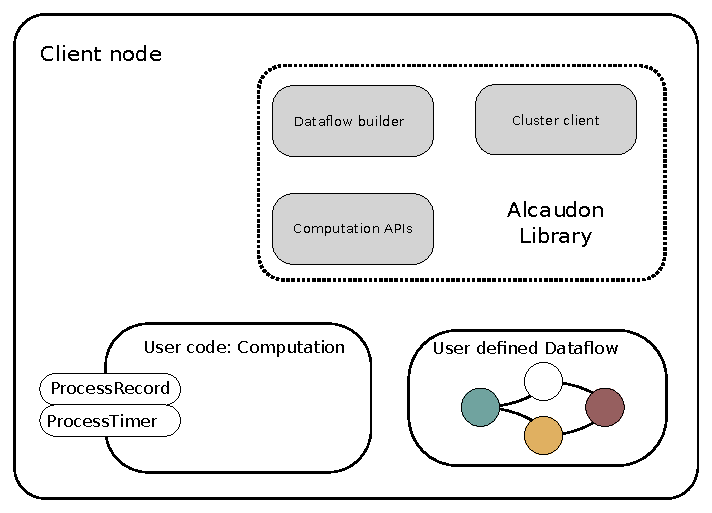
\includegraphics[width=0.6\textwidth]{client.pdf}
  \caption{Alcaudon library}
  \label{fig:library}
\end{figure}

This library is composed of 3 modules as it is shown in figure~\ref{fig:library}:

\begin{itemize}
\item Computation API's: Interface that users should implement in order to
  create computations.
\item Dataflow builder: This component is used to build dataflow topologies and
  later on submit the to the cluster coordinator.
\item Cluster client: Communication layer between clients and Alcaudon clusters.
  It handles all the operations needed to submit custom code to the cluster as well
  as the stream processing pipeline definition.
\end{itemize}

\subsubsection{Computation API's}

As it was explained before, in order to create custom computations to process
unbounded data-sets in Alcaudon, it is necessary to implement an interface. The
interface is listed in~\ref{code:computation}. As it can be observed there are
to methods to implement; \lstinline[columns=fixed]{processRecord(record:
  Record)} and \lstinline[columns=fixed]{processTimer(timer: Timer)}. These methods
are the main entry point into user code.

\begin{lstlisting}[language=scala, frame=trBL, label=code:computation, float=ht, caption = {Computation API's}]
case class RawRecord(value: Array[Byte], timestamp: Long) {
  val id = UUID.randomUUID().toString
}
case class Record(key: String, rawRecord: RawRecord) {
  val value = rawRecord.value
  val timestamp = rawRecord.timestamp
  val id = UUID.randomUUID().toString
}
\end{lstlisting}


\begin{lstlisting}[language=scala, frame=trBL, label=code:computation, float=ht, caption = {Computation API's}]
trait Computation
    extends ProduceAPI
    with TimerAPI
    with StateAPI
    with SerializationAPI
    with RuntimeContext {
  ...
  def processRecord(record: Record): Unit
  def processTimer(timer: Timer): Unit
  ...
}
\end{lstlisting}

\begin{lstlisting}[language=scala, frame=trBL, label=code:auxiliarcomputation, float=ht, caption = {Auxiliary computation API's}]
trait ProduceAPI { environment: RuntimeContext =>
  protected def produceRecord(record: RawRecord, stream: String): Unit =
}

trait TimerAPI { environment: RuntimeContext =>
  protected def setTimer(timer: Timer): Unit
}

trait StateAPI { environment: RuntimeContext =>
  protected def set(key: String, value: Array[Byte]): Unit
  protected def get(key: String): Array[Byte]
}

trait SerializationAPI {
  def serialize[T](data: T)(implicit ti: TypeInfo[T]): Array[Byte]
  def deserialize[T](binary: Array[Byte])(implicit ti: TypeInfo[T]): T
}
\end{lstlisting}

